\documentclass[12pt,oneside,a4paper]{article}
\usepackage[utf8]{inputenc}
\usepackage[hidelinks]{hyperref}
\usepackage[english]{babel}
\usepackage{indentfirst}
\usepackage{graphicx}
\usepackage[font=small,skip=0pt]{caption}
\usepackage{tocloft}
\renewcommand{\cftsecleader}{\cftdotfill{\cftdotsep}}
\renewcommand{\baselinestretch}{1.5}
\def\labelitemi{--}

\usepackage{geometry}
 \geometry{
    a4paper,
    left=20mm,
    right=10mm,
    top=20mm,
    bottom=20mm,
 }

\let\oldenumerate\itemize
\renewcommand{\itemize}{
  \oldenumerate
  \setlength{\itemsep}{0pt}
  \setlength{\parskip}{0pt}
  \setlength{\parsep}{0pt}
}

\title{Openlab - Automated testing and evaluation platform of the source code from assignments}
\author{Mihai Iachimovschi}
\date{}

\begin{document}
\maketitle
\clearpage

\renewcommand*\contentsname{Table of contents}
\tableofcontents
\clearpage

\listoffigures
\clearpage
 
\listoftables
\clearpage

\section{Project Analysis and System Requirements}
\subsection{Project analysis}
Openlab is a platform which aims to provide automated testing and evaluation of students based on their source code from the assignments. The goal of the system is to offer the possibility to organize the assignments for any subject in order to make them easily accessible for both students and teachers. It offers a transparent layer for setting strict deadlines, penalization for late submissions and even rewards for early submissions. Also, speaking of transparency, for any assignment there is a open grading policy which includes the requirements list and the points a student can achieve. Thus, it is intended to improve the efficiency coefficient of students and professors.

The system has a web interface which makes it extremely flexible and cross-platform. The UI is simplified as much as possible so it can be used by anyone without additional training. From the student's perspective, the system will run on his code a prepared test case that was written by the professor and will publish it's results. All the external code should be executed in a completely isolated environment in order to protect the server from malicious code that can be submitted.

Conceptually speaking, the core of Openlab can be described as a platform which can accommodate fully isolated containers that compile and execute all the provided source code, saving the results to a database.

\subsubsection{Problem description}
Students from the IT faculty are dealing with a lot of laboratory works, homeworks and individual assignments for which they should implement different algorithms by writing small programs. For each subject, the requirements are presented in varying forms which makes a inconsistent work-flow for both students and teachers.

Scheduled laboratory sessions become focused on verification and evaluation of students' past assignments. This activity is very time consuming for the professor and it turns out that almost all the time reserved for the lab is consumed by this important but time-wasting procedure.

Automated testing and evaluation of the source code can obviously improve the learning process by focusing on more important and useful tasks. Professors can spend more time on explaining different approaches, technologies or algorithms that can be used for the assignments instead of verifying past assignments in the time reserved for the lab class.

People tend to procrastinate, that's why a lot of students submit their assignments late. Not having a obvious overview of the deadlines can be misleading for students. Being confused may leave space for excuses. That's why enforcing transparent deadlines,notifications and bonuses for early submissions may improve student's punctuality which is useful not only in university.

\subsubsection{Overview of similar products}
Most of the similar projects position themselves as LMS (Learning Management System). The main goal of learning management systems is the delivery of electronic educational materials to the students. It offers also to the professors a way to administer and document courses and also track students' results by evaluating assignments and tests.

\textbf{Moodle} is a flexible, free software, open-source learning platform. It is a LMS that offers basic assignment submission features, forum for discussions, glossary of definitions, a taxonomy for courses and lectures and on-line quiz module. Moodle is written in PHP and can be deployed on any server capable of running PHP and it requires a web server such as Apache or NGiNX. It is compatible with MySQL, PostgreSQL and other relational database management systems.

\textbf{DigitalChalk} is a proprietary Learning Management System which allow users to create and deliver their courses materials on-line. The solution is provided to the customers as a SaaS (Software as a Service). The price starts at 4.95\$ per month per user with an initial setup fee starting at 399\$.

\textbf{Blackboard Learning System} is a complex proprietary Learning Management System. It is highly customizable and it can be either deployed on local server or used as SaaS. The company's pricing policy is not publicly available, however it is rated as expensive.

All considered applications are great tools, highly functional and useful, but none of them has the possibility of automatic testing and evaluation of source code for the assignments which is very important for IT faculty. 

Some of the similar products offer too much overhead in terms of unneeded functional while others are too expensive for a non-profit organization. Openlab aims to provide a minimalistic and simplistic approach to the problem solving. It is also Free and Open Source Software.

\subsection{System requirements}
\subsubsection{Product functions}
This section provides a brief overview of the functions that system will perform. Below are presented the key functions of the product which must be implemented in the final version. The whole system should have the following features:
\begin{itemize}
  \item Keep track of laboratory assignments for users (students);
  \item System should accept assignment submissions and evaluate them;
  \item System should provide an interface for professors for adding new assignments and test cases;
  \item Execute safely the submitted code and the test and save the results;
  \item Grade automatically the submitted and executed assignments;
  \item Inform students about last changes via a private feed;
  \item Display upcoming assignments for logged in student;
  \item Display upcoming laboratory sessions;
  \item Display enrolled courses that registered in the system;
  \item Keep track of grades from the automatically graded assignments;
\end{itemize}

\subsubsection{Constraints and dependencies}
This sections presents basic requirements for the whole ecosystem. A client that uses the applications has to have a modern web browser installed on his system. On the back-end side, constraints and dependencies are the following:
\begin{itemize}
  \item Server should run any Linux distribution with kernel newer than 3.10;
  \item Docker 1.4 or newer should be installed;
  \item Python 2.7 or newer should be installed;
  \item Python PIP should be installed. It will provide packages as: fig, virtualenv, django, etc.;
  \item TCP ports :80 and :443 should be available;
\end{itemize}

\subsubsection{User questions for information system}
The user interface represents the space by which user interacts with the system in order to benefit from system's features. It should provide instant feedback for user's actions. It should also give us the answers of predefined questions:
\begin{itemize}
  \item What are the upcoming assignments?
  \item What are the deadlines for the future assignments?
  \item For when is scheduled the next laboratory session?
  \item What are the enrolled courses?
  \item What is the amount of credits obtained by a specific subject?
  \item What are the grades for specific subject?
  \item What are the requirements of specific assignment?
  \item Which are the results of my previous submissions?
  \item How many submission trials are left?
  \item What is the highest score obtained for a specific assignment?
\end{itemize}

\subsubsection{User interface requirements}
This section presents the description of the interface, which should create the bigger picture of how the platform should look like. The main goal is to keep interface as clean and minimalistic as possible. The three main views can be seen in: Figure \ref{fig:mock_up_dashboard}, Figure \ref{fig:mock_up_feed} and Figure \ref{fig:mock_up_assignment}.

For best results we should take into account these aspects:
\begin{itemize}
  \item All visual elements that provide key functionalities should be easily accessible;
  \item The User Interface should have a steep learning curve;
  \item The interface should avoid ambiguity by making everything clear with text or graphical elements;
  \item Responsiveness should be guaranteed;
  \item The interface should be engineered in a forgiving way such that the user should be better notified about the potential mistake rather than punished;
  \item The interface should not be bloated with irrelevant nor redundant elements.
\end{itemize}

\begin{figure}[!ht]
  \centering
    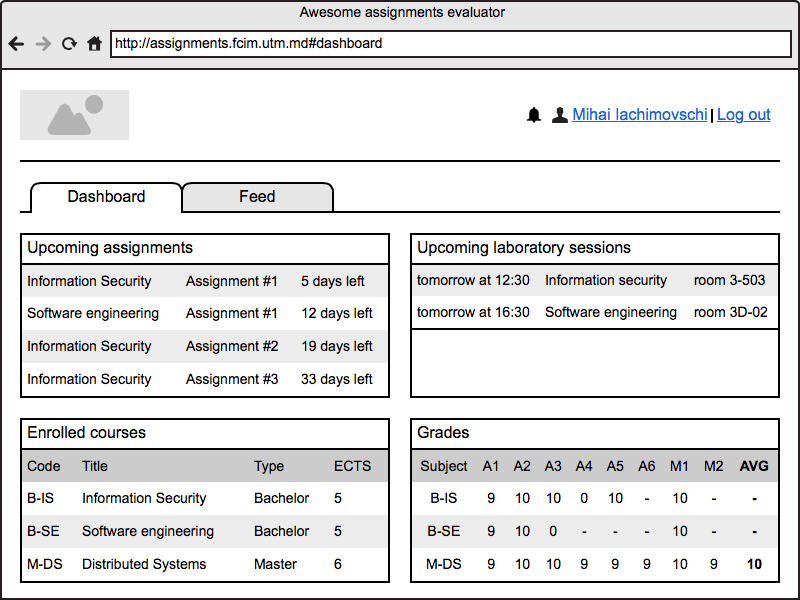
\includegraphics[width=0.9\textwidth]{pic/wireframe-dashboard.png}
    \caption{Graphical User Interface mock-up for the dashboard page.}
    \label{fig:mock_up_dashboard}
\end{figure}

In Figure \ref{fig:mock_up_dashboard} is represented the page with the user's dashboard. The content from this page is split in four regions that makes an overview of the current state of the user. The four zones provide to the user information about: upcoming assignments, upcoming laboratory sessions, enrolled courses and obtained grades.

This page has the purpose of giving an informative snapshot of the state of student in his relation with the Openlab system. It offers an easy way of visualization of all the details organized on a single page which aims to help the user to make decisions regarding his time-management and also to evaluate the past productivity level.

\begin{figure}[!ht]
  \centering
    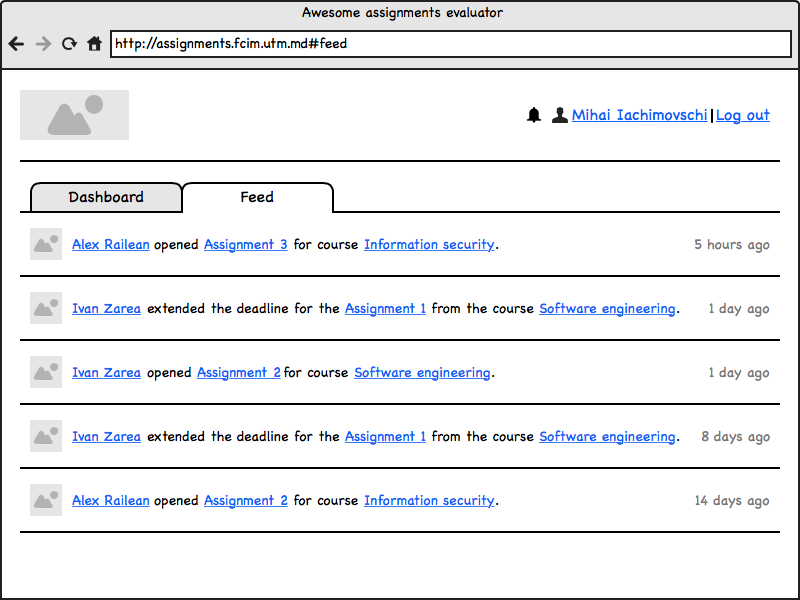
\includegraphics[width=0.9\textwidth]{pic/wireframe-feed.png}
    \caption{Graphical User Interface mock-up for the feed page.}
    \label{fig:mock_up_feed}
\end{figure}

Figure \ref{fig:mock_up_feed} represents the user interface of the feed page. The content of this page is organized in a simple and minimalistic way, taking advantage of white-space. On this view user can find a relevant overview of the activity regarding his enrolled courses. The list of past events is sorted by the date of event, so the most fresh one is on the top of the list. Also, the user have access to navigate directly from the feed to the specified course, assignment or professor's page by hyper-links.

\begin{figure}[!ht]
  \centering
    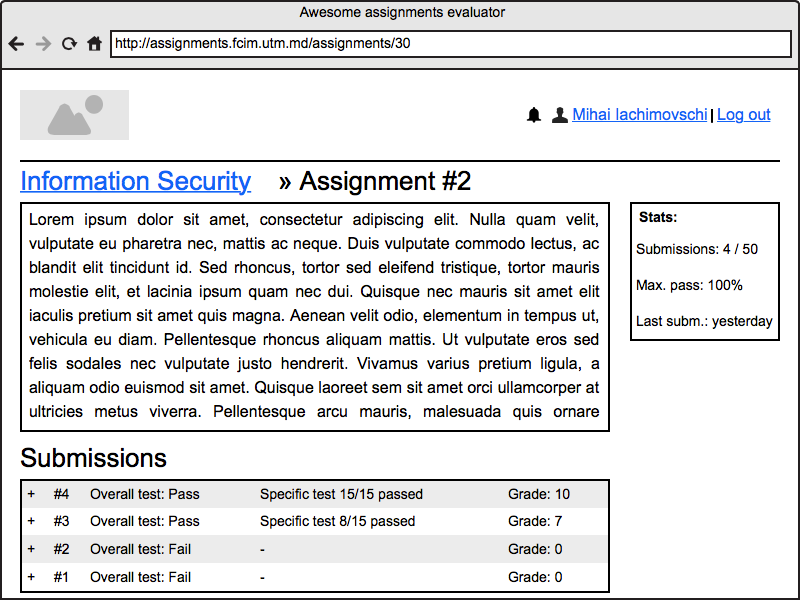
\includegraphics[width=0.9\textwidth]{pic/wireframe-assignment.png}
    \caption{Graphical User Interface mock-up for the assignment page.}
    \label{fig:mock_up_assignment}
\end{figure}

Figure \ref{fig:mock_up_assignment} displays the most functional-dependent page that provide useful information and also has a call to action which provides to the user the possibility to submit his work. The view is designed such that it provides the detailed information about the assignment requirements and this piece of information occupies the most of the space. Also, there is a widget with brief statistics about user's success and progress on current assignment. There is also a section which gives us detailed information about each past submission -- visible on user's action.

\section{Software Modeling}

\section{System Implementation}

\subsection{Project localization}

\end{document}